% LaTeX .tex
% Example for the proceedings of the  25th International Congress of Mechanical Engineering
% COBEM 2019
% October, 20-25, 2019, Uberlândia, MG, Brazil
% Based on the template of the proceedings of COBEM2015 and COBEM2017

\documentclass[10pt,fleqn,a4paper,twoside]{article}
\usepackage{abcm}
\def\shortauthor{Ian Costa Alves, Felipe José Oliveira Ribeiro and Alexandre Zuquete Guarato}
\def\shorttitle{Dynamic Modeling of a Rocket for High Accuracy Trajectory Simulations}
\usepackage{subcaption}
\captionsetup{compatibility=false}
\usepackage{blindtext}
\usepackage{amsmath}
\usepackage{mathtools}
\begin{document}
\fphead
\hspace*{-2.5mm}\begin{tabular}{||p{\textwidth}}
\begin{center}
\vspace{-4mm}
\title{Modelagem dinâmica do voo de um foguete para simulações de trajetória de alta exatidão}
\end{center}
\authors{Ian Costa Alves} \\
\authors{Felipe Jose Oliveira Ribeiro} \\
\authors{Alexandre Zuquete Guarato}\\
\institution{Federal University of Uberlândia (UFU), Av. João Naves de Ávila, 2121, Campus Santa Mônica, Uberlândia, MG } \\
\institution{iancostalves@gmail.com} \\
\institution{feliperibeiro.ufu@gmail.com} \\
\institution{azguarato@ufu.br} \\
\\
\abstract{\textbf{Abstract.} For the design of an aerospace vehicle, high fidelity flight simulations are essential and can be critical to enable or invalidate the product. In the case of rockets and missiles this becomes even more critical, since the exact location of the landing site is a determining parameter for launch planning. In this paper, a dynamic modeling with six degrees of freedom for the flight of a rocket is discussed, as well as a consistent aerodynamic model based on the Extended Barrowman's Method for obtaining the aerodynamic forces and moments for the rocket flight. In addition to the modeling, results of flight simulations will be shown with the proposed model.}\\
\\
\keywords{\textbf{Keywords:} Aerospace, Rocket, Dynamic simulations, Trajectory simulation, Flight mechanics}\\
\end{tabular}

%\section{INTRODUCTION}
%
%Uma modelagem dinâmica de complexidade física e matemática aceitável, mas que ainda assim descreva de forma satisfatória os eventos da realidade é uma busca constante em inúmeros ramos da engenharia. Para o ramo aeroespacial não é diferente, sempre há maneiras de tornar um modelo mais fiel, mas muitas vezes a complexidade que essa alteração acrescenta torna uma modelagem mais simples preferível.
%
%+blablabla

\section{INTRODUCTION}

%O projeto de veículos aeroespaciais é tido como uma atividade de alta complexidade. O forte carácter multidisciplinar desta atividade resulta em uma constante busca por referencias nas mais diversas áreas da engenharia. Para uma prática segura deste tipo de projeto grande atenção técnica deve ser investida desde as concepções teóricas no início da missão até as partes práticas finais de construção. Para isso, estudos devem ser feitos de forma a se ter sob controle o maior número de variáveis possível, minimizando assim a probabilidade de falhas. 

The design of aerospace vehicles is seen as a highly complex activity. The strong multidisciplinary character of this field results in a constant research for references in the most diverse areas of engineering. For a safe practice of this type of project, great technical attention must be invested all the way from the theoretical conceptions at the beginning of the mission to the final construction of the parts. For this, studies must be done in order to have as many variables as possible under control, thus minimizing the probability of failure.

%O estudo da dinâmica de um mini foguete tem grande importância, visto que possibilita a avaliação de propriedades cinemáticas como velocidade máxima, apogeu e dispersão horizontal ao fim do voo, além das principais solicitações mecânicas experimentadas pela estrutura a partir das acelerações impressas no veículo durante sua trajetória. Para tal, cria-se um modelo representativo da realidade onde se aplicam as forças e as leis de balanço. Tais equações diferenciais são então integradas numericamente, resultando na trajetória e nos esforços simulados. 

The study of the dynamics of a mini rocket has great importance, since it allows the evaluation of kinematic properties such as maximum speed, apogee and horizontal dispersion at the end of the flight. Besides that is possible to achieve the main mechanical stress experienced by the structure from maximum accelerations throw the trajectory. For this, a representative model of reality is created where forces and laws of balance are applied. These differential equations are then numerically integrated, resulting in a simulated experiment.


%Tendo esse objetivo em mente, no presente trabalho, busca-se desenvolver esse modelo de forma acurada, considerando-se a influencia das forças mais significativas que agem sobre um modelo foguete durante o voo, como a força gravitacional, os esforços aerodinâmicos e o empuxo advindo do motor. Para modelar tais grandezas utilizou-se o modelo de Barrowman na aerodinâmica, aproximações experimentais para o empuxo e um modelo linearizado da gravidade.

With this objective in mind, in the present paper,we aim to develop this model accurately, considering the influence of the most significant forces acting on a rocket model during flight, such as gravitational force, aerodynamic forces and thrust coming from the engine. To model such quantities, the Barrowman model was used in aerodynamics, experimental approaches for thrust and a linearized gravity model was considered.


%Ao fim do estudo se pretende comparar as simulações com testes materiais desenvolvidos pela Equipe de Propulsão e Tecnologia Aeroespacial (EPTA) da UFU, como forma de validação.  

At the end of the study it is intended to compare the simulations with material tests developed by the Aerospace Technology and Propulsion Team (EPTA) of UFU, as a form of validation.

\section{METHODOLOGY}
% Para o desenvolvimento da dinâmica do foguete, primeiramente, foi determinado um modelo físico tanto para o foguete quanto para o espaço circundante. Foram então fixados eixos de referencia e matrizes de conversão de grandezas vetoriais entre estes eixos. Por último sendo definidos os modelos das forças atuantes. Após isso, houve a discretização do tempo e a integração numérica da equação resultando em um modelo teórico completo.

For the development of rocket dynamics, a physical model was first determined for both the rocket and the surrounding space. Reference axes and conversion matrices were then established between these axes. Finally, the models of the acting forces are defined. After this, time was discretized and the numerical integration of the equation resulted in an approximated result.

\subsection{Physical model}
%O foguete foi considerado como um corpo rígido de massa constante. O referencial cartesiano também considerou o planeta terra como plano, e a gravidade com módulo e sentido constantes na vertical para baixo durante toda a trajetória do veículo. A geometria do foguete pode ser descrita de acordo com a Fig. (\ref{geometria_foguete}).

The rocket was considered as a rigid body of constant mass. The Cartesian referential also considered the earth as plane, and gravity with modulus and direction constant vertically downward throughout all the trajectory of the vehicle. The geometry of the rocket can be described according to Fig. (\ref{geometria_foguete}).

\begin{figure}[h!]
	\centering
	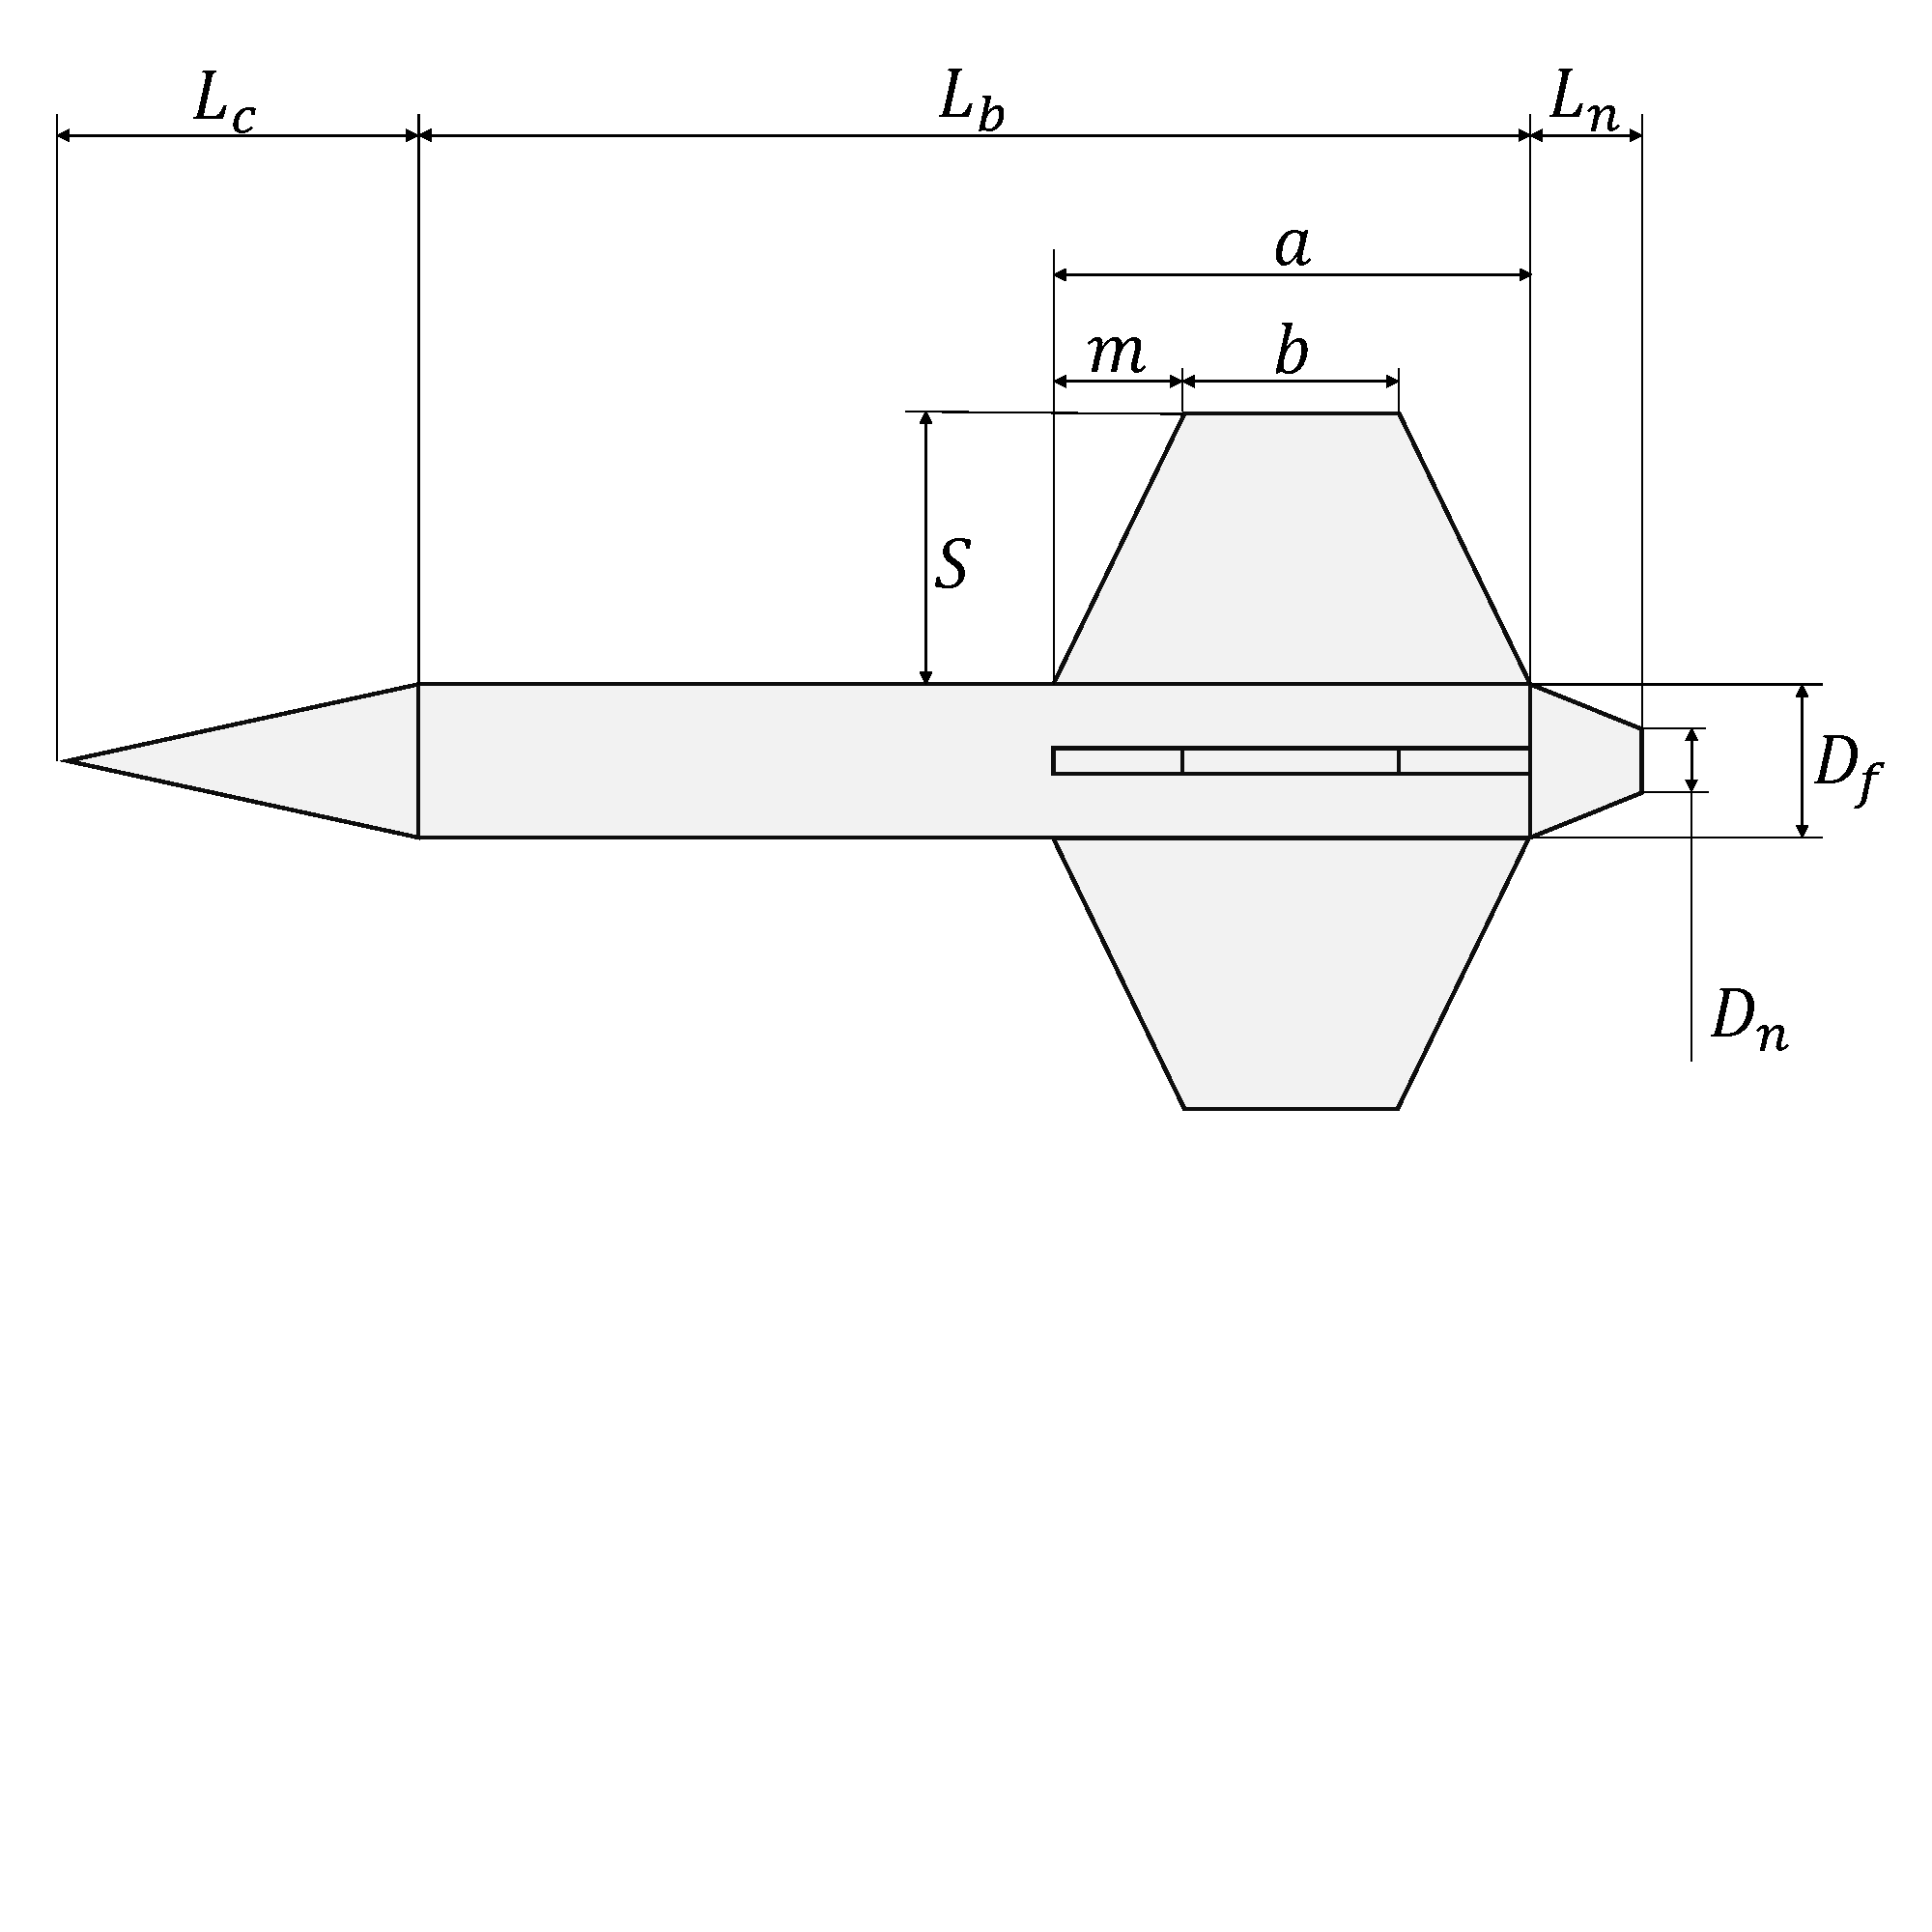
\includegraphics[trim = {0cm 13cm 0cm 0cm}, clip , angle=0, scale=0.15]{imagens/foguete_statera}
	\caption{Outward geometry of the rocket.}
	\label{geometria_foguete}
\end{figure}
n this geometry, the fins were considered as flat plates with a maximum thickness of 10 percent of the lowest chord line.



\subsubsection{Reference axes and transfer matrices}
%Para se descrever a dinâmica do sistema é necessária a criação de três eixos de referencia espaciais: eixo inercial ($ _{I} $), eixo do corpo ($ _{B} $) e eixo dos ventos ($ _{W} $).

In order to describe the dynamics of the system it is necessary to create three spatial reference axes: Inertial frame ($ _{I} $), body frame ($ _{B} $) and wind frame ($ _{W} $).

%O eixo inercial é fixo em um ponto da terra, com o eixo Z apontando para baixo, adotaremos a origem do sistema como a origem do lançamento. O eixo do corpo tem origem no centro de gravidade (CG) do corpo e rotaciona junto com ele, de modo que o eixo x coincide com o eixo longitudinal do foguete. Por último temos o eixo dos ventos, cuja origem também está no CG do corpo, porém o eixo x coincide com a direção do vetor velocidade do veículo. Uma representação dos eixos de referência pode ser observada na Fig. (\ref{ref_foguete}).

The inertial axis is fixed at a point on the earth, with the Z axis pointing downward, we will adopt the origin of the system as the origin of the launch. The axis of the body originates in the center of gravity (CG) of the body and rotates along with it, so that the x-axis coincides with the longitudinal axis of the rocket. Finally we have the axis of the winds, whose origin is also in the CG of the body, but the x axis coincides with the direction of the vehicle speed vector. A graphical representation of the reference axes can be seen in Fig. (\ref{ref_foguete}).


\begin{figure}[h!]
	\centering
	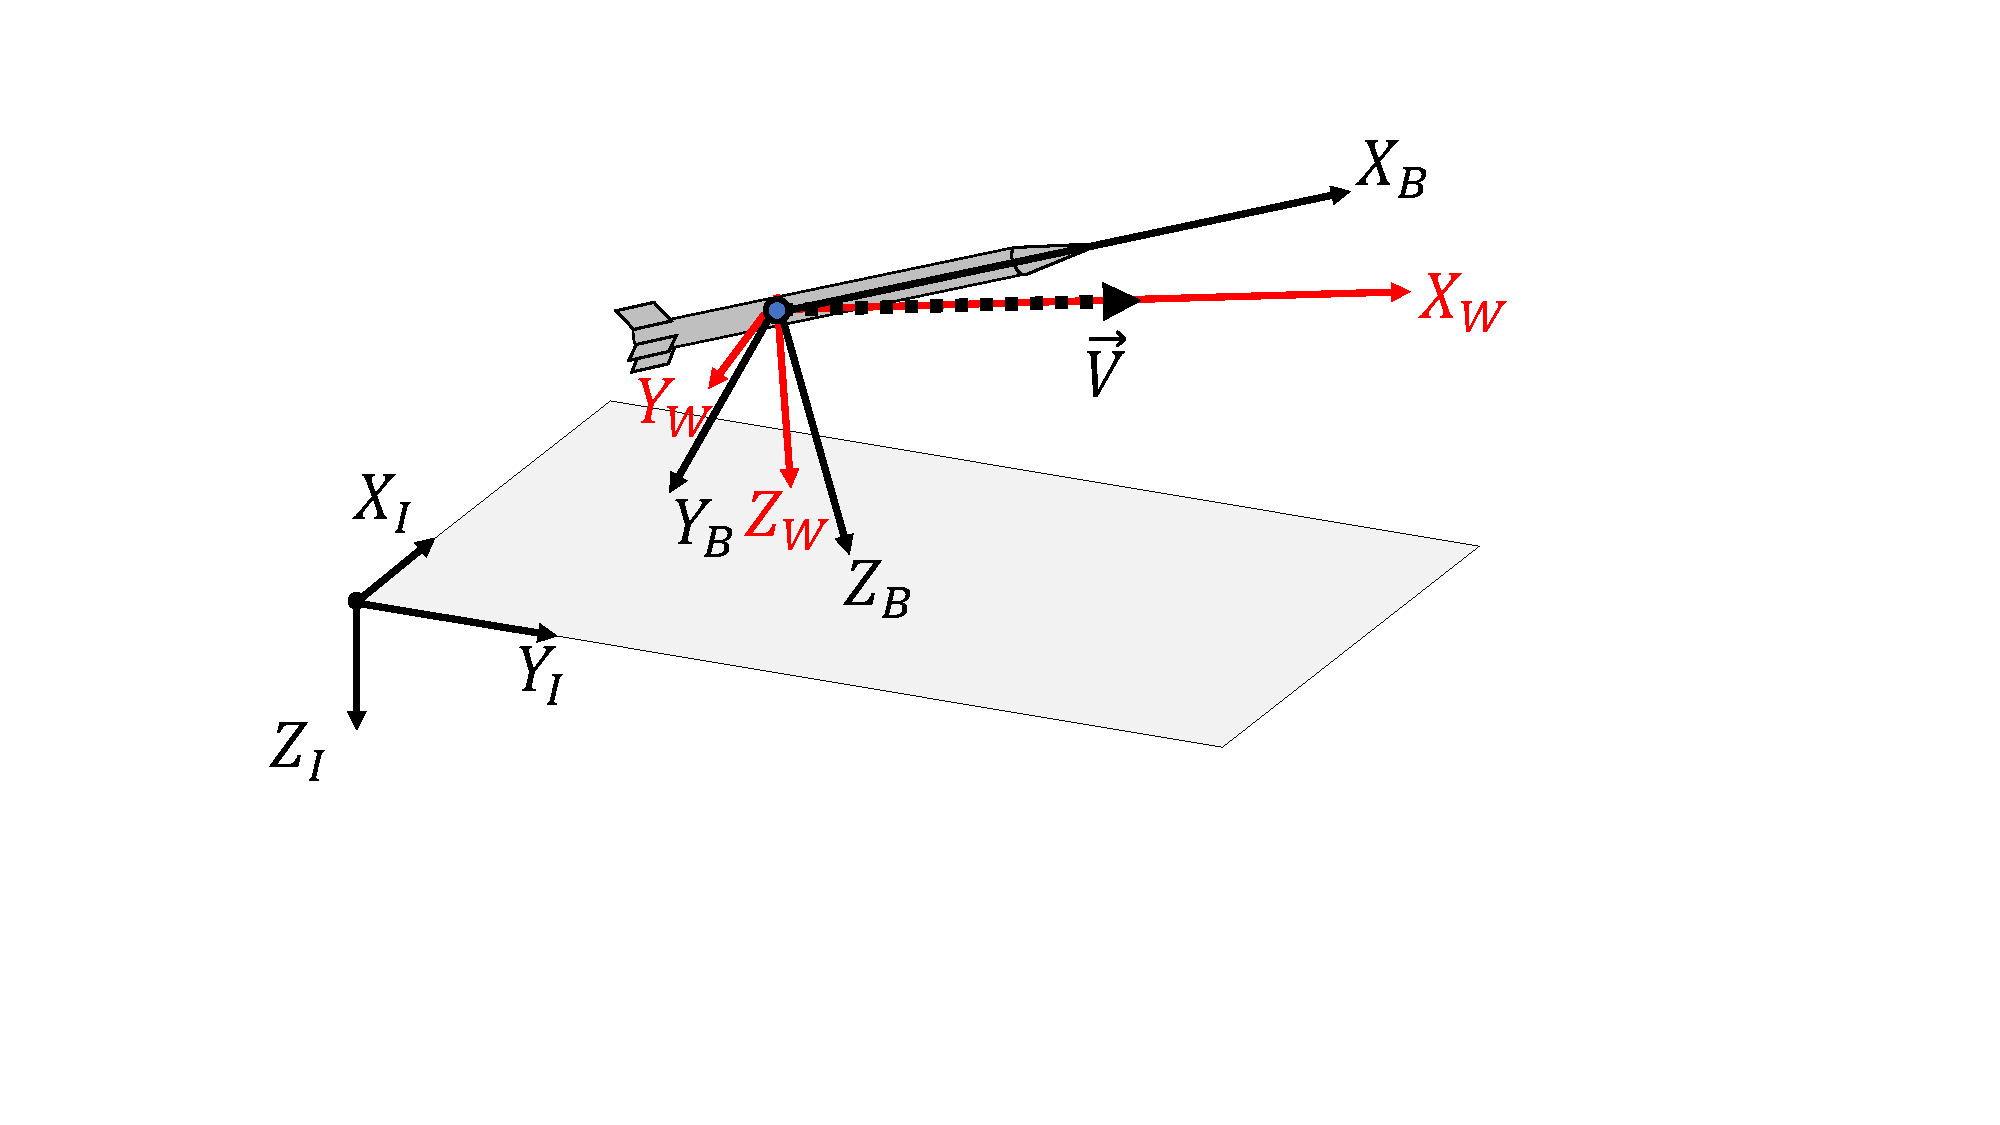
\includegraphics[trim = {4cm 5cm 8cm 1cm}, clip , angle=0, scale=0.3]{imagens/eixos_referencia}
	\caption{Reference frames in the flight of a rocket.}
	\label{ref_foguete}
\end{figure}

%Com os eixos de referencia explicitados usaremos matrizes de transformação com ângulos específicos para explicitar a relação entre cada um deles. Os ângulos de Euler ($ \Phi, \Theta, \Psi $) são usados para relacionar os eixos inercial e do corpo, podendo ser observados na Fig. ().

With the axes of reference determined, transformational matrices with specific angles will be used. The angles of Euler ($ \Phi, \Theta, \Psi $) are used to relate the inertial and body axes, and can be observed in Fig. (\ref{angulos}).

\begin{figure}[h!]
	\centering
	\begin{subfigure}[t]{0.29\textwidth}
	\centering
	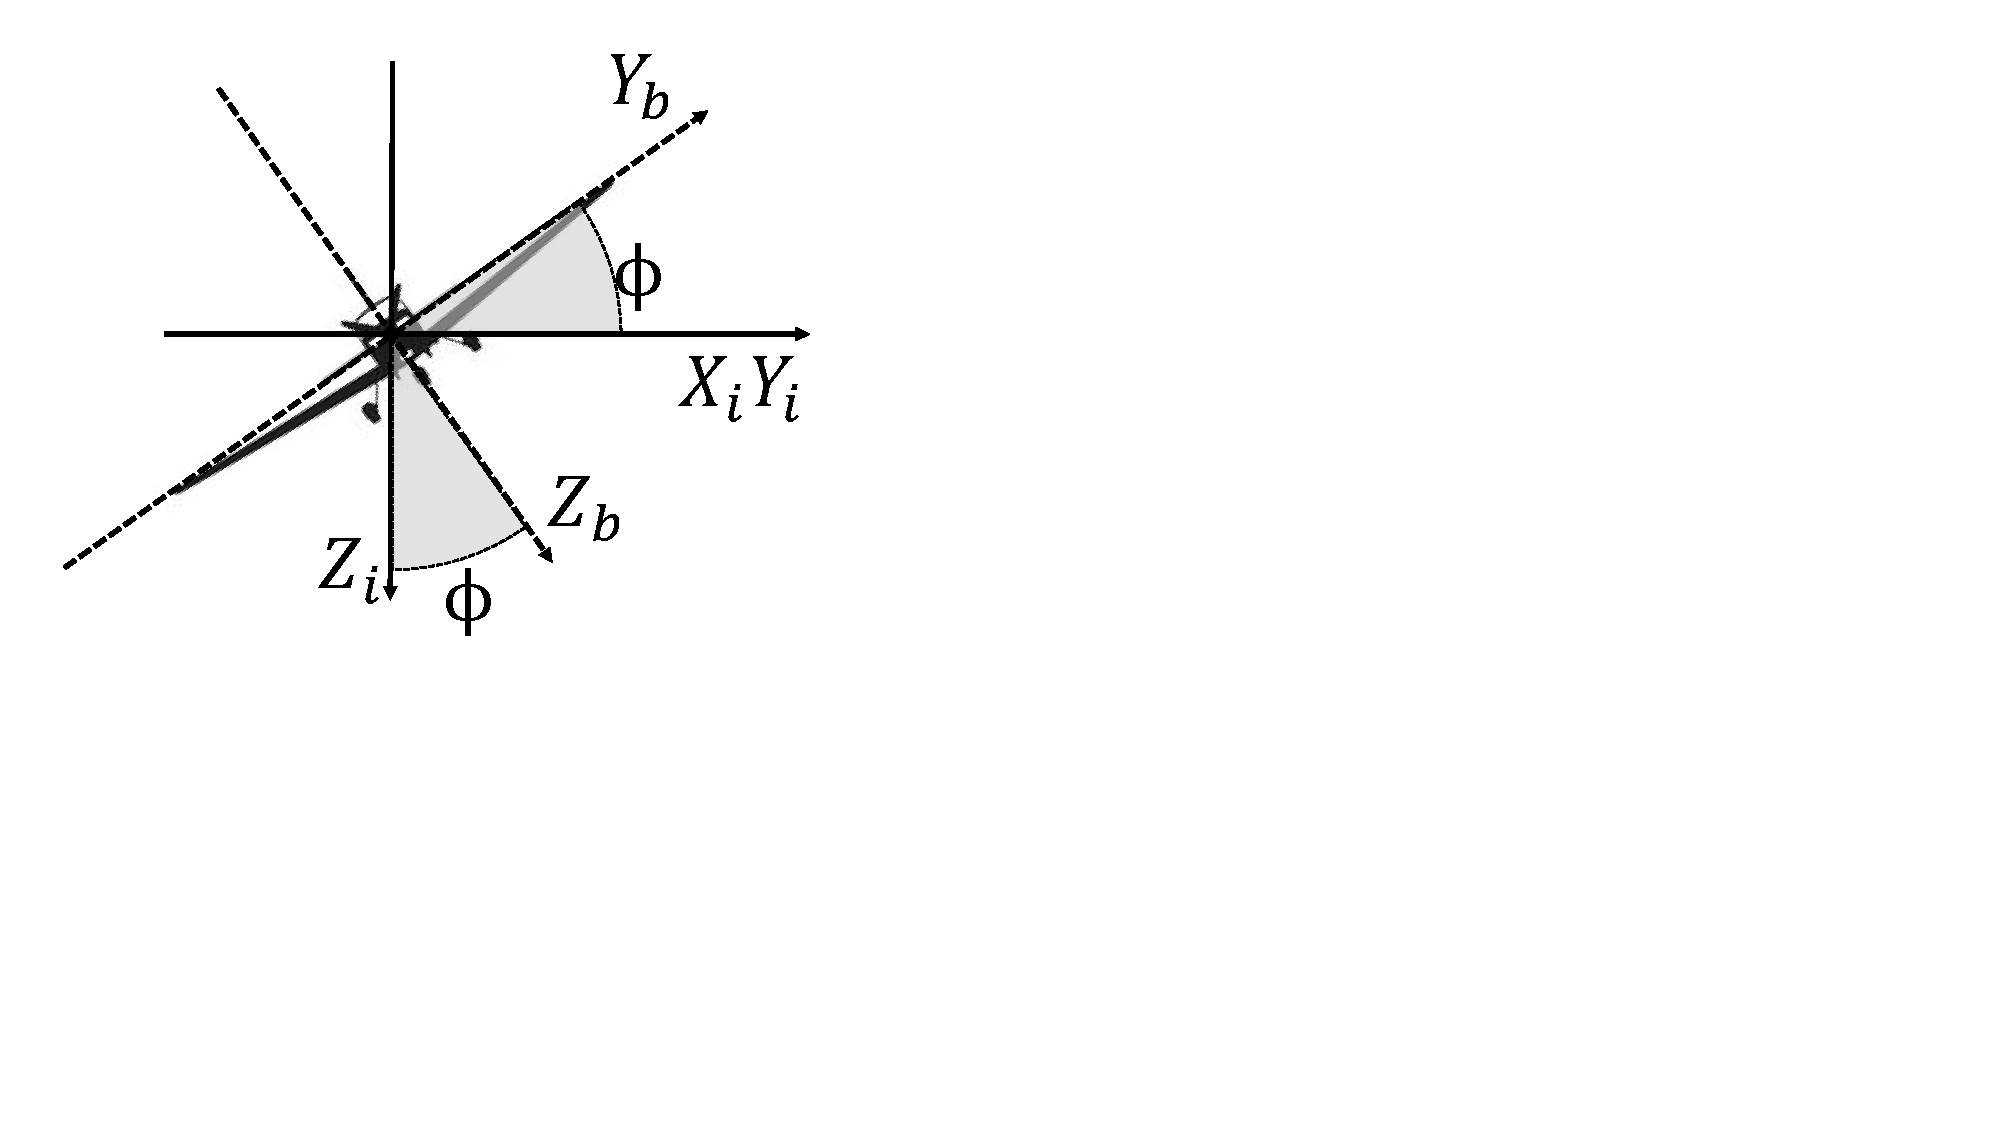
\includegraphics[trim = {0cm 6.5cm 0cm 0cm}, clip, angle=0, scale=0.25]{imagens/angulos_foguete_phi}	
	\caption{Roll Angle.}
	\end{subfigure}
	\begin{subfigure}[t]{0.29\textwidth}
		\centering
		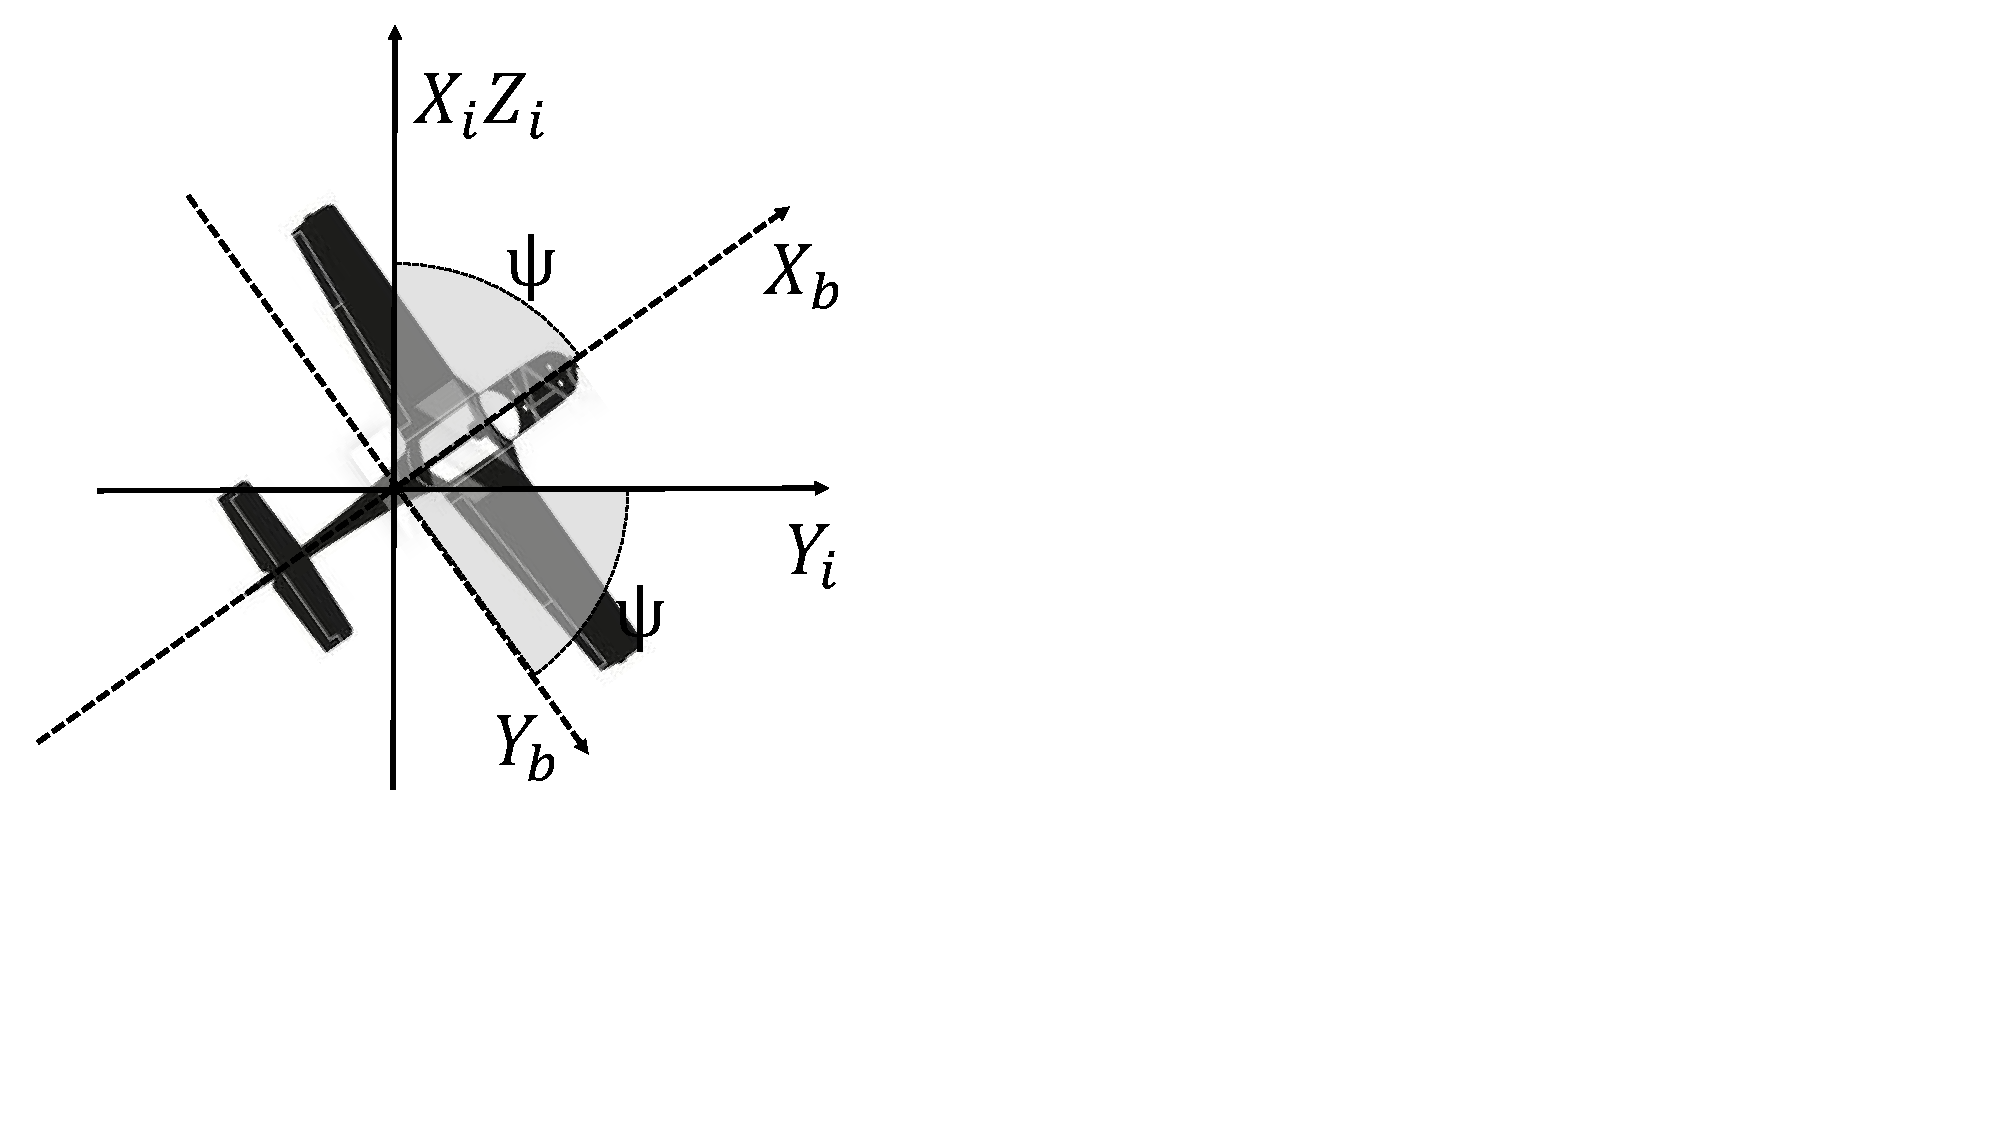
\includegraphics[trim = {0cm 4cm 0cm 0cm}, clip, angle=0, scale=0.25]{imagens/angulos_foguete_Psi}	
		\caption{Yaw angle.}
	\end{subfigure}
	\begin{subfigure}[t]{0.29\textwidth}
		\centering
		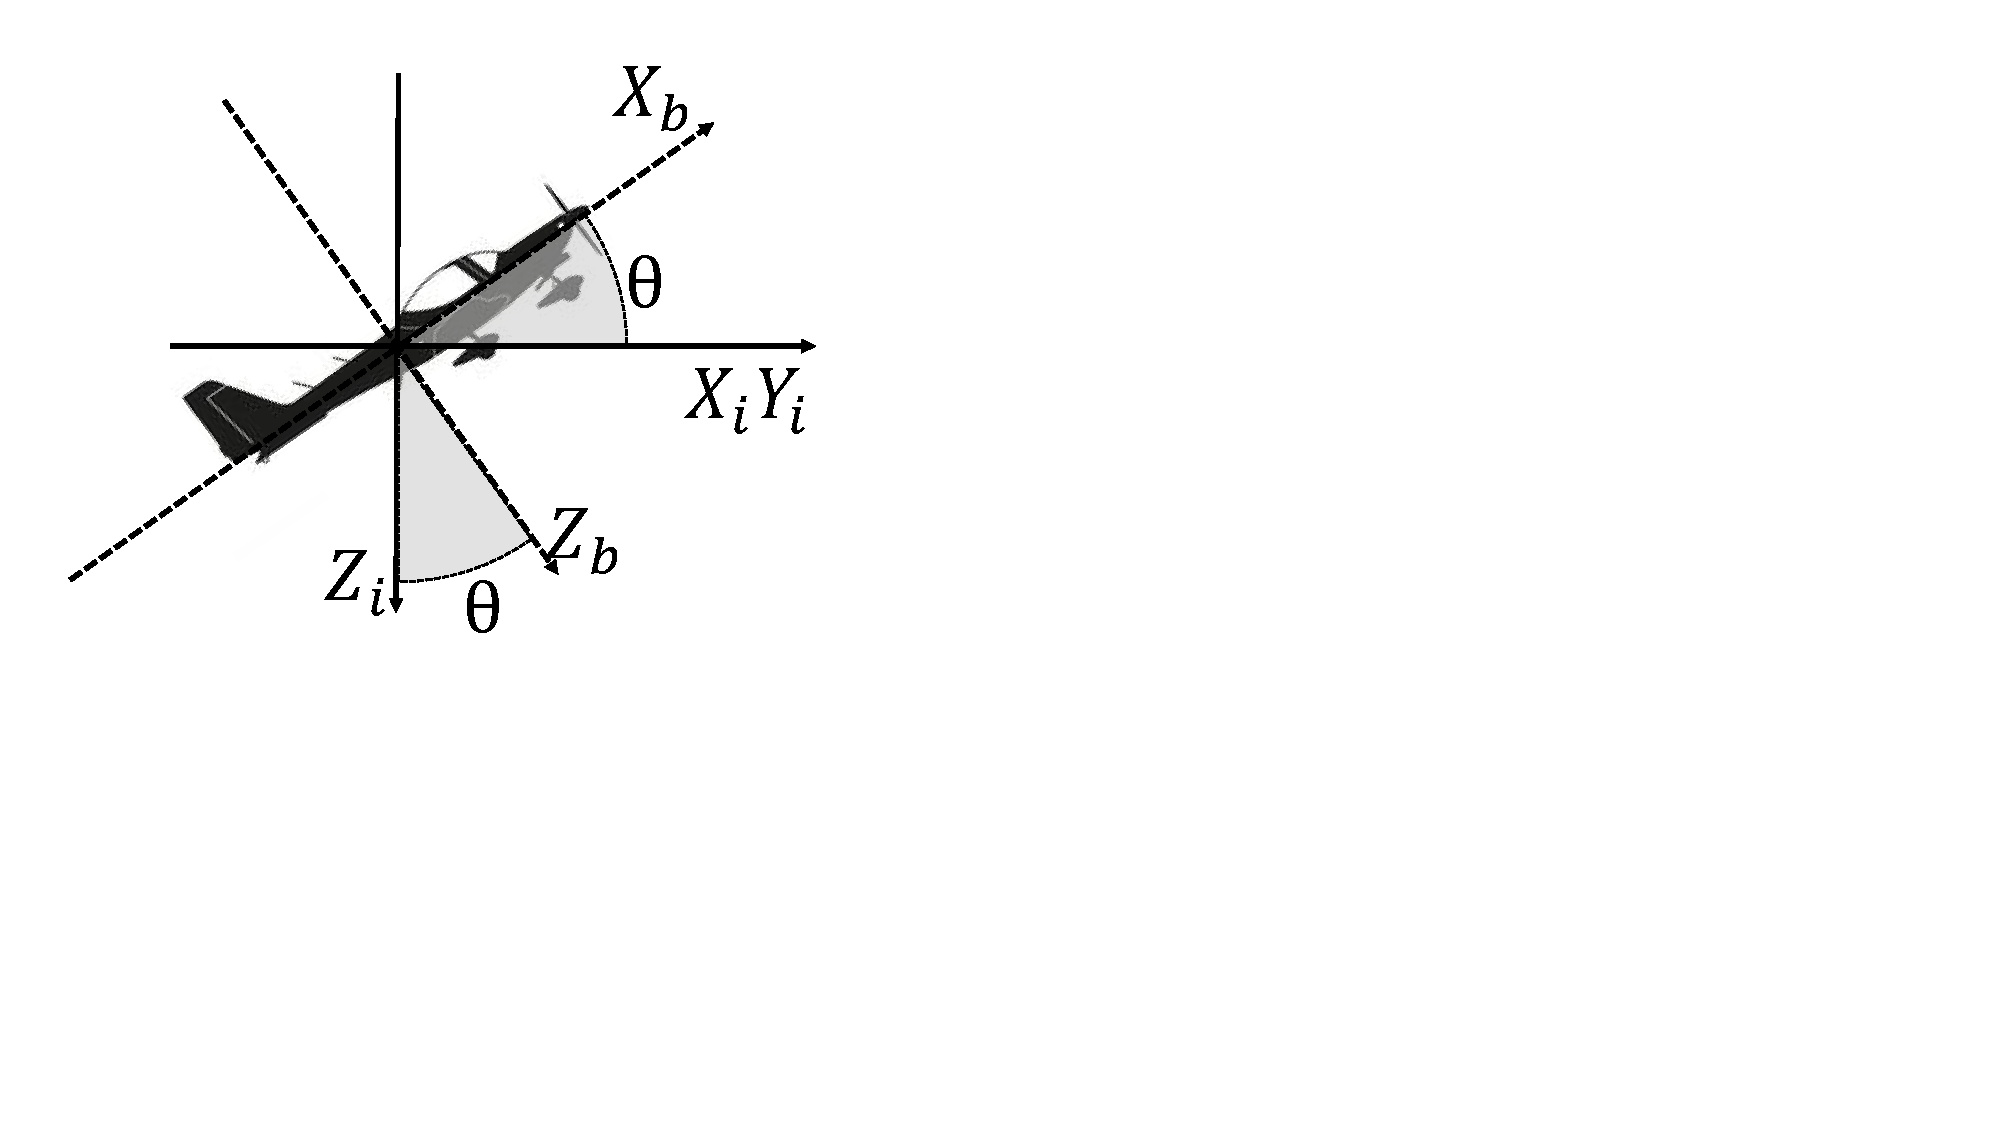
\includegraphics[trim = {0cm 6.5cm 0cm 0cm}, clip, angle=0, scale=0.25]{imagens/angulos_foguete_theta}	
		\caption{Pitch angle.}
	\end{subfigure}
\label{angulos}
\caption{Euler angles.}
\end{figure}

%Desse modo, podemos escrever a matriz de transformação do eixo do corpo para o eixo inercial bem como sua inversa, como explicita a Eq. (\ref{BtoI}).

In this way, we can write the transformation matrix of the axis of the body to the inertial axis as well as its inverse, as written on Eq. (\ref{BtoI}).

\begin{equation}
\mathcal{L}_{IB}=
\begin{bmatrix}
\cos\Theta\cos\Psi & \sin\Psi\sin\Theta\cos\Psi-\cos\Phi\sin\Psi & \cos\Phi\sin\Theta\cos\Psi+\sin\Phi\sin\Psi\\
\cos\Theta\sin\Psi & \sin\Psi\sin\Theta\sin\Psi+\cos\Phi\cos\Psi & \cos\Phi\sin\Theta\sin\Psi-\sin\Phi\cos\Psi\\
\sin\Theta & \sin\Phi\cos\Theta & \cos\Phi\cos\Theta\\
\end{bmatrix}=\mathcal{L}_{BI}^{-1}
\label{BtoI}
\end{equation}




\subsubsection{Dynamic model for a 6 DOF rocket}
%Uma vez desenvolvidas as relações cinemáticas, é necessário o desenvolvimento das equações dinâmicas para o movimento do veículo. Para isso, partimos de duas equações fundamentais: a equação do balanço da quantidade movimento linear (Eq. (\ref{balancolinear})) e a equação do balanço da quantidade de movimento angular (Eq. (\ref{balancoangular})) na forma generalizada para um corpo rígido.


Once the kinematic relations are developed, it is necessary to develop the dynamic equations for the motion of the vehicle. For this, we start from two fundamental equations: the equation of the balance of linear momentum (Eq. (\ref{balancolinear})) and the equation of balance of angular momentum (Eq. (\ref{balancoangular})) in generalized form to a rigid body.


\begin{equation}
{m}\left( \frac{\partial \vec{V}}{\partial t}\right)_{B}+\vec{\omega}\times \vec{V}=\vec{F} 
\label{balancolinear}
\end{equation}

\begin{equation}
\int_{V} \vec{r}\times (\vec{\omega}\times \vec{r})+\vec{\omega}\times(\vec{\omega}\times \vec{r})  \rho \ dV = \vec{M}
\label{balancoangular}
\end{equation}

%Onde $\vec{F}$ é o somatório das forças aerodinâmicas, peso e empuxo (Eq. (\ref{forcas})) e $\vec{M}$ é o somatório dos momentos de cada uma dessas forças em torno da origem do sistema de coordenadas do corpo.

Where $ \vec{F} $ is the sum of the aerodynamic forces, weight and thrust (Eq.(\ref{forcas})) and $\vec{M}$ is the sum of the angular momentum of each of these forces around origin of the body coordinate system.



\begin{equation}
\vec{F}=\vec{W}+\vec{A}+\vec{T}
\label{forcas}
\end{equation}

\begin{equation}
\vec{M}=\vec{M}_{W}+\vec{M}_{A}+\vec{M}_{T}
\label{momentos}
\end{equation}

%Fazendo a manipulação da Eq. (\ref{balancolinear}) e separando nos três eixos do corpo, obtemos as Eqs. (\ref{fx}), (\ref{fy}) e (\ref{fz}).

By manipulating Eq. (\ref{balancolinear}) and separating the three axes of the body, we obtain Eqs. (\ref{fx}), (\ref{fy}) and (\ref{fz}):


\begin{equation}
m(\dot{U}-V\ R+W\ Q)=F_{x}
\label{fx}
\end{equation}
\begin{equation}
m(\dot{V}+U\ R-W\ P)=F_{y}
\label{fy}
\end{equation}
\begin{equation}
m(\dot{W}-U\ Q+V\ P)=F_{z}
\label{fz}
\end{equation}

Doind the same with Eq.(\ref{balancoangular}) and assuming that the xy and xz planes are planes of mass symmetry, we obtain the Eqs. (\ref{mx}), (\ref{my}) e (\ref{mz}).

\begin{equation}
I_{xx}\dot{P}+(I_{zz}-I_{yy})R\ Q=M_{x}
\label{mx}
\end{equation}
\begin{equation}
I_{yy}\dot{Q}+(I_{xx}-I_{zz})P\ R=M_{y}
\label{my}
\end{equation}
\begin{equation}
I_{zz}\dot{R}+(I_{yy}-I_{xx})P\ Q=M_{z}
\label{mz}
\end{equation}

\subsubsection{Thrust and Weigth}

%Em comparação com as forças aerodinâmicas, empuxo e peso são forças muito mais simples de serem calculadas, bem como os momentos gerados por elas. Considerando que não há vetorização de empuxo, podemos descrever o empuxo com a Eq. (\ref{empuxo}).

In comparison to aerodynamic forces, thrust and weight are much simpler forces to calculate, as well as the moments generated by them. Considering that there is no vectorization of thrust, we can describe the thrust with:


\begin{equation}
\vec{T}= 
\begin{bmatrix}
\ T \\
0\\
0 \\
\end{bmatrix}
_{B}
\label{empuxo}
\end{equation}

%De modo que $ T $ varia no tempo conforme uma dada curva de empuxo, na Fig. (\ref{thrustcurve}) é mostrada a curva de empuxo do motor Estes D12 para fins de exemplificação.

So that $ T $ varies in time according to a given thrust curve. 

Now, for the weight, making the approximation of the earth as flat, we can describe the force with the Eq. (\ref{peso}).

\begin{equation}
\vec{W}=m\vec{g}=m
\begin{bmatrix}
0\\0\\g\\
\end{bmatrix}_{I}=m\ \mathcal{L}_{BI}
\begin{bmatrix}
0\\0\\g\\
\end{bmatrix}_{I}=m
\begin{bmatrix}
-g\sin\Theta \\
g\sin\Phi\cos\Theta \\
g\cos\Phi\cos\Theta \\
\end{bmatrix}_{B}
\label{peso}
\end{equation}

\subsubsection{Aerodynamic model}
%Com as equações dinâmicas e o modelo de empuxo prontos, nos resta somente modelar as forças e momentos provenientes da interação do airframe com o escoamento externo e é isso que será desenvolvido nesta seção.

With the dynamic equations and the thrust model ready, we have only to model the forces and moments from the interaction of the airframe with the external flow and this is what will be developed in this section.

%Uma forma de resolver o problema seria acoplar o modelo dinâmico a um código de CFD transiente, de modo a obter com a rotina de CFD as forças e momentos que o fluido aplica no airframe do foguete em cada instante de tempo. Todavia a complexidade e o custo computacional inviabilizam tal aplicação.

One way to solve the problem would be to couple the dynamic model to a transient CFD code in order to obtain with the CFD routine the forces and moments that the fluid applies to the rocket airframe at each instant of time. However, complexity and computational cost make such application inviable.

%Desse modo, utilizaremos o método de Barrowman extendido para o cálculo dos coeficientes aerodinâmicos do foguete. O método utilizado foi desenvolvido em (REFERENCIA BARROWMAN), que separa cada uma das estruturas externas do foguete e calcula a força que o escoamento exerce em cada uma, assim como mostra a Fig. (\ref{aeroforces}).

Thus, we will use the extended Barrowman method to calculate the aerodynamic coefficients of the rocket. The method was developed in (REFERENCIA BARROWMAN), which separates each of the outer structures of the rocket and calculates the force that the flow exerts on each one, as shown in Fig. (\ref{aeroforces}).

\begin{figure}[h!]
	\centering
	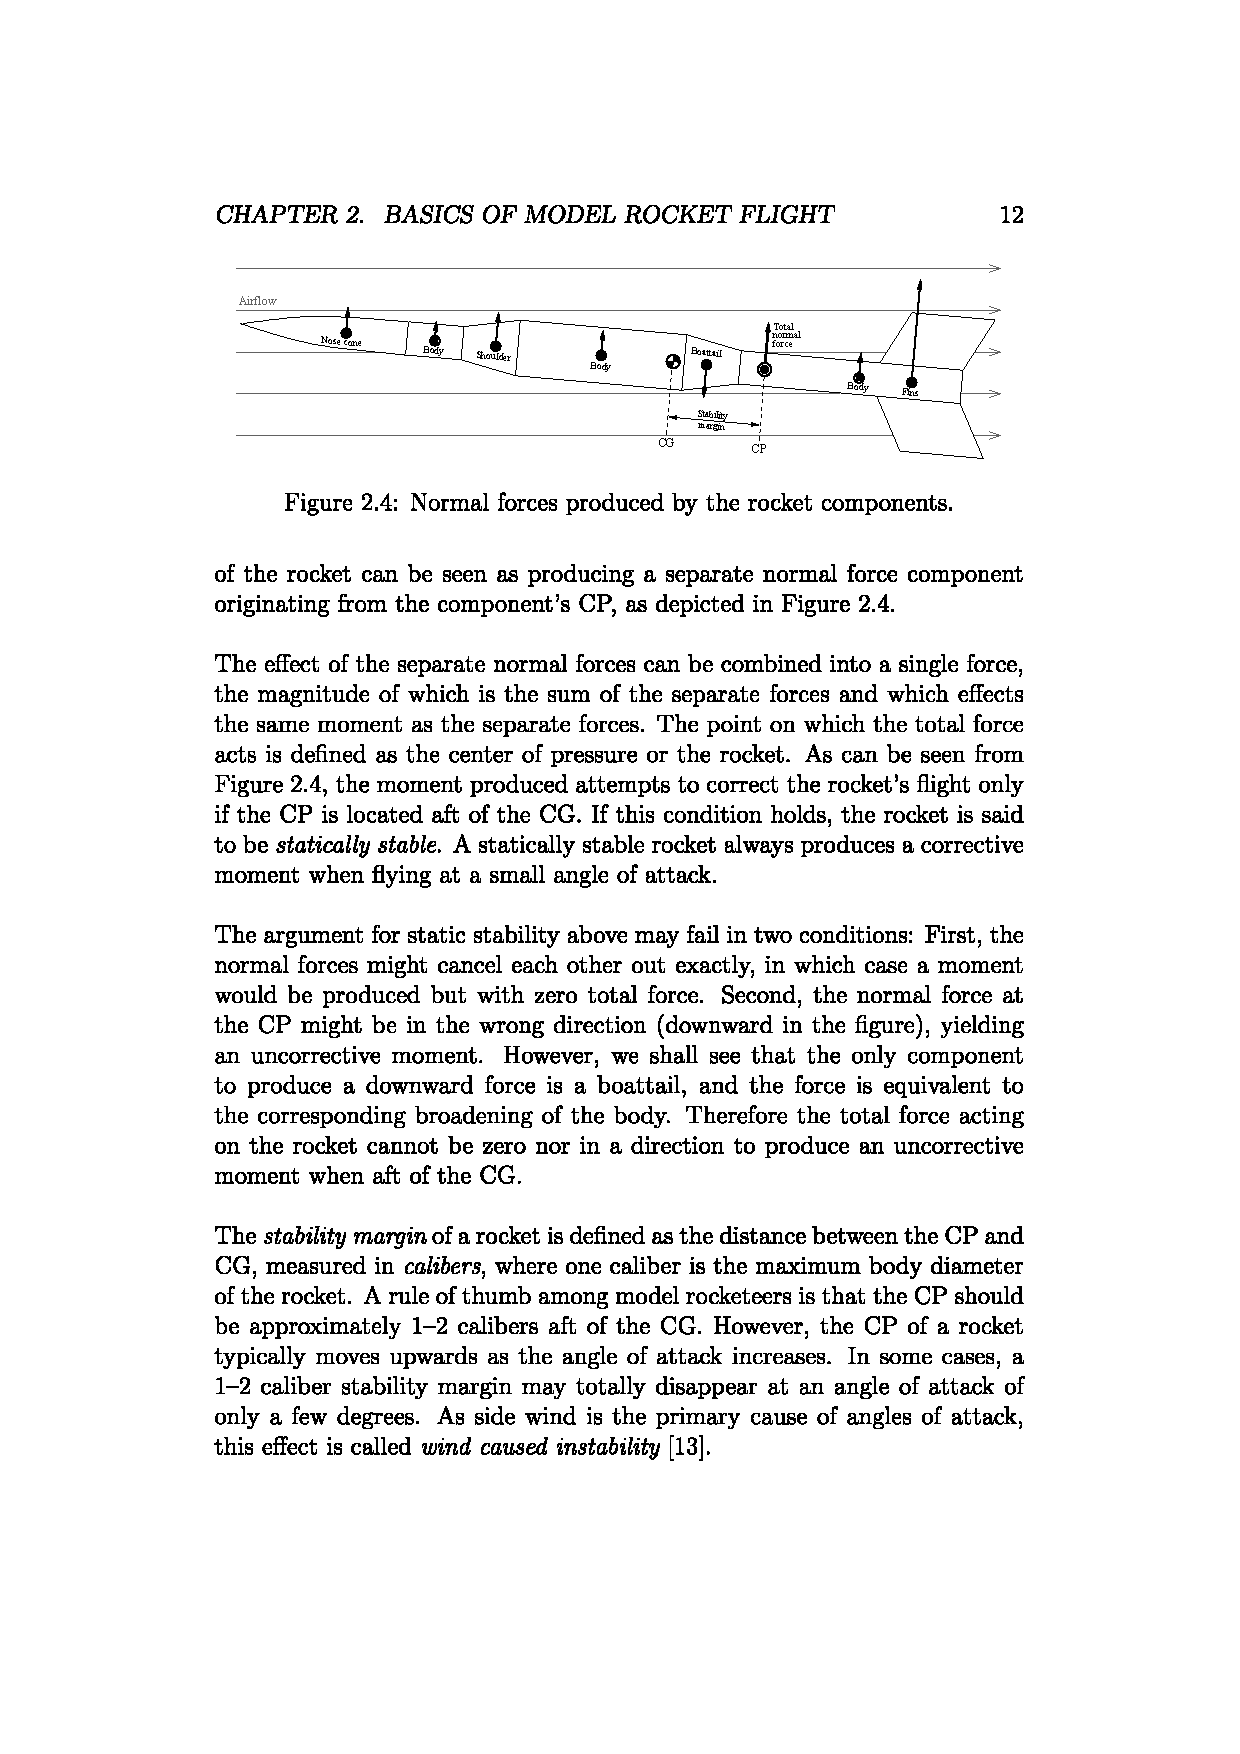
\includegraphics[angle=0, trim={3cm 21.5cm 3cm 4cm}, clip, scale=0.7]{imagens/aeroforces}
	\caption{Figura ilustrativa das forças aerodinâmicas atuando no foguete}
	\label{aeroforces}
\end{figure}

%Considerando que o ângulo de ataque não ultrapasse 15 graus, podemos usar a relação mostrada na Eq. (\ref{cnalpha}) para equacionar a força normal em cada uma das estruturas aerodinâmicas.

Considering that the angle of attack does not exceed 15 degrees, we can use the ratio shown in Eq. (\ref {cnalpha}) to equate the normal force in each of the aerodynamic structures.

\begin{equation}
\vec{A}=\sum_{i}\vec{A}_{(i)}=\sum_{i}
\begin{bmatrix}
-A_{(i)} \\
Y_{(i)} \\
-Z_{(i)} \\
\end{bmatrix}
_{B} = \sum_{i} \rho (\pi D_{f}^{2})V_{wind}^{2}
\begin{bmatrix}
-C_{A (i)} \\
C_{Y (i)} \\
-C_{Z (i)} \\
\end{bmatrix}
_{B} = \sum_{i} \rho (\pi D_{f}^{2})V_{wind}^{2}
\begin{bmatrix}
-C_{A (i)} \\
C_{N_{\alpha} (i)}\beta_{(i)} \\
-C_{N_{\alpha} (i)}\alpha_{(i)} \\
\end{bmatrix}
_{B}
\label{cnalpha}
\end{equation}

%Onde $ A $, $ Y $ e $ Z $ são respectivamente a força axial, força normal Y e força normal Z de cada um dos componentes. Com isso, o método mencionado fornece um equacionamento para o coeficiente de força normal ($ C_{N_{\alpha}} $) de cada um dos componentes, em função da geometria dos componentes e do número de mach ($ Ma $) do escoamento, bem como a posição do centro de pressão (CP) de cada uma delas. Com isso é possível o cálculo do momento total em torno do CG com a Eq. (\ref{somatoriom}).

Where $ A $, $ Y $ and $ Z $ are respectively the axial force, normal force Y and normal force Z of each of the components. Thereby, said method provides an equation for the normal force coefficient ($ C_{N_{\alpha}} $) of each of the components, as a function of the geometry of the components and mach number ($ Ma $) of the the center of pressure (CP) of each of them. With this it is possible to calculate the total momentum around the CG with Eq. (\ref{somatoriom}).


\begin{equation}
\vec{M}_{A}=\sum_{i} \vec{M}_{A (i)}=\sum_{i} (\vec{r}_{(i)}\times \vec{A}_{(i)})
= \sum_{i}  
\begin{bmatrix}
x_{(i)} \\
0\\
0\\
\end{bmatrix}
_{B} \times
\begin{bmatrix}
-A_{(i)} \\
Y_{(i)} \\
-Z_{(i)} \\
\end{bmatrix}
_{B}= \sum_{i} 
\begin{bmatrix}
M_{x (i)} \\
x_{(i)}Z_{(i)} \\
x_{(i)}Y_{(i)} \\
\end{bmatrix}
_{B}
\label{somatoriom}
\end{equation}

%Onde $ \vec{r_{(i)}} $ é a posição do CP de cada estrutura escrita no referencial do corpo. O método também propõe um equacionamento do momento em torno do eixo x do corpo ($ M_{x} $) em função da geometria do foguete, do $ Ma $ e da velocidade de rotação em torno de x ($ P $), que será detalhado no paper final.


Where $ \vec{r_{(i)}} $ is the position of the CP of each structure written in the frame of the body. The method also proposes an equation of the moment around the x-axis of the body ($ M_{x} $) as a function of the rocket geometry, $ Ma $ and the speed of rotation around x ($ P $), which will be detailed in the final paper.


\subsection{Mathematical and computational model}


\section{ACKNOWLEDGEMENTS}

The authors would like to thank the following professors and institutions: FEMEC (Faculdade de Engenharia Mecânica), UFU (Universidade Federal de Uberlândia) and, especially, EPTA (Equipe de Propulsão e Tecnologia Aeroespacial) for financial support.




\section{REFERENCES} 

\bibliographystyle{abcm}
\renewcommand{\refname}{}
\bibliography{bibfile}

\end{document}
